\documentclass[12pt]{article}

\usepackage{answers}
\usepackage{setspace}
\usepackage{graphicx}
\usepackage{enumitem}
\usepackage{multicol}
\usepackage{mathrsfs}
\usepackage[margin=1in]{geometry} 
\usepackage{amsmath,amsthm,amssymb}
\usepackage[ngerman]{babel}

\newcommand{\N}{\mathbb{N}}
\newcommand{\Z}{\mathbb{Z}}
\newcommand{\C}{\mathbb{C}}
\newcommand{\R}{\mathbb{R}}

\DeclareMathOperator{\sech}{sech}
\DeclareMathOperator{\csch}{csch}

\newenvironment{theorem}[2][Theorem]{\begin{trivlist}
		\item[\hskip \labelsep {\bfseries #1}\hskip \labelsep {\bfseries #2.}]}{\end{trivlist}}
\newenvironment{definition}[2][Definition]{\begin{trivlist}
		\item[\hskip \labelsep {\bfseries #1}\hskip \labelsep {\bfseries #2.}]}{\end{trivlist}}
\newenvironment{proposition}[2][Proposition]{\begin{trivlist}
		\item[\hskip \labelsep {\bfseries #1}\hskip \labelsep {\bfseries #2.}]}{\end{trivlist}}
\newenvironment{lemma}[2][Lemma]{\begin{trivlist}
		\item[\hskip \labelsep {\bfseries #1}\hskip \labelsep {\bfseries #2.}]}{\end{trivlist}}
\newenvironment{exercise}[2][Exercise]{\begin{trivlist}
		\item[\hskip \labelsep {\bfseries #1}\hskip \labelsep {\bfseries #2.}]}{\end{trivlist}}
\newenvironment{solution}[2][Solution]{\begin{trivlist}
		\item[\hskip \labelsep {\bfseries #1}]}{\end{trivlist}}
\newenvironment{problem}[2][Problem]{\begin{trivlist}
		\item[\hskip \labelsep {\bfseries #1}\hskip \labelsep {\bfseries #2.}]}{\end{trivlist}}
\newenvironment{question}[2][Question]{\begin{trivlist}
		\item[\hskip \labelsep {\bfseries #1}\hskip \labelsep {\bfseries #2.}]}{\end{trivlist}}
\newenvironment{corollary}[2][Corollary]{\begin{trivlist}
		\item[\hskip \labelsep {\bfseries #1}\hskip \labelsep {\bfseries #2.}]}{\end{trivlist}}

\begin{document}
	\title{Künstliche Intelligenz 2 - Zusammenfassung}
	\author{Michael Gabler}
	\maketitle
	\tableofcontents
	\newpage
	
	\section{Unsicheres Wissen und Schließen}
	Logik benötigt exakte Regeln, die immer wahr sind. Oft nicht gegeben (zu wenig Daten, keine Regeln möglich) $\rightarrow$ wahrscheinlichkeitsbasiertes Entscheiden. Ein Agent benötigt dazu Präferenzen, wie nützlich verschiedene Ziele sind und die Wahrscheinlichkeiten, diese Ziele zu erreichen.\\
	\textbf{Rationalität} = wähle Aktion mit der größten erwarteten Nützlichkeit
	
	\subsection{Wahrscheinlichkeitsrechnung}
	\textbf{unbedingte Wahrscheinlichkeit} $P(A)$\\
	\textbf{Wahrscheinlichkeitsverteilung} $P(Wetter) = (0,7; 0,2; 0,008; 0,02)$\\
	\textbf{Operanden} $\wedge$ = und, $\vee$ = oder\\
	\textbf{Bedingte Wahrscheinlichkeit} wie wahrscheinlich ist $A$ wenn $B$ wahr ist:
	$$P(A|B) = \frac{P(A \wedge B)}{P(B)} \Leftrightarrow P(A \wedge B) = P(A|B) P(B)$$\\
	$P(A \vee B) = P(A) + P(B) - P(A \wedge B)$\\
	\textbf{Apriori-Wahrscheinlichkeit} Wahrscheinlichkeit für ein Ereignis unabhängig von den anderen: $P(X) = \sum_y P(X,y)$ (Marginalization) oder $P(X) = \sum_y P(X|y) P(y)$ (Conditioning)\\
	\textbf{Unabhängige Variablen} Für Variablen, deren Ereignisse unabhängig voneinander eintreten gilt: $P(a|b) = P(a)$\\
	\textbf{Bayes' Theorem} $P(B|A) = \frac{P(A|B) P(B)}{P(A)}$ wird verwendet zur Herleitung nicht bekannter, abhängiger Wahrscheinlichkeiten\\
	\textbf{Naives Theorem von Bayes} Annahme: Symptome $S_i$ untereinander unabhängig (oft nicht gegeben), Vollständigkeit der Diagnosen $D_i$
	$$P(D_i|S_1 \wedge ... \wedge S_m) = \frac{P(D_i) P(S_1|D_i) ... P(S_m|D_i)}{\sum_{j=1}^{n} P(D_j) P(S_1|D_j) ... P(S_m|D_j)} = \alpha P(D_i) P(S_1|D_i) ... P(S_m|D_i)$$
	Dabei ist $\alpha$ eine Normierungskonstante, so dass die Summer aller Wahrscheinlichkeiten 1 ergibt.\\
	\textbf{Numerische Variablen} Annahme: alle Variablen haben diskrete Werte. Kontinuierliche Variablen werden diskretisiert oder Verwendung, wenn Verteilungsfunktion bekannt ist.
	
	\subsection{Probabilistische/Bayessche Netze}
	Theorem von Bayes behandelt alle Symptome als voneinander unabhängig. Probabilistische Netze (gerichtete, azyklische Graphen) stellen Abhängigkeiten dar.\\
	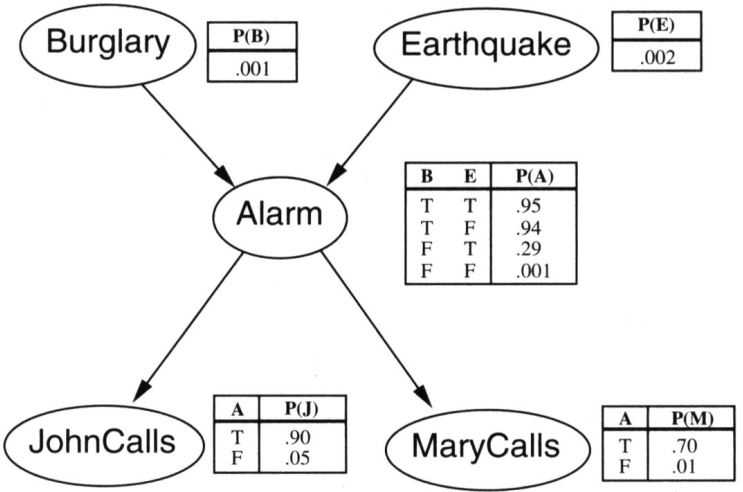
\includegraphics[width=\textwidth]{figures/probabilistisches-netz.JPG}\\
	\textbf{Konstruktion von probabilistischen Netzen}
	\begin{enumerate}
		\item Wähle geeignete Zufallsvariable
		\item Wähle Reihenfolge der Variablen (Wichtig für Größe des Netzes)
		\item Solange Variablen noch nicht im Netz sind:
			\subitem Nimm nächste Variable $X_i$
			\subitem Setze die Eltern von $X_i$ auf eine minimale Menge von bereite im Netz vorhandenen Knoten
			\subitem Definiere die Wahrscheinlichkeitstabelle für $X_i$
	\end{enumerate}
	Es ermöglicht die Wahrscheinlichkeitsberechnung jeder vollständigen Knotenbelegung.\\
	Beispiel: $$P(J \wedge M \wedge A \wedge \bar{B} \wedge \bar{E}) = P(J|A) P(M|A) P(A|\bar{B} \wedge \bar{E}) P(\bar{B}) P(\bar{E}) = 0,9 \cdot 0,7 \cdot 0,0001 \cdot 0,999 \cdot 0,998 = 0,000628$$
	\textbf{Enumerate-Joint-Ask} Berechnung von nicht vollständigen Knotenbelegungen $\rightarrow$ bilde Summe über unbekannte Möglichkeiten: $$P(B|J \wedge M) = \alpha P(B,J,M) = \alpha \sum_e \sum_a P(B \wedge e \wedge a \wedge J \wedge M)$$
	$\Rightarrow$ Komplexität für $n$ boolsche Variablen: $O(n2^n)$\\
	\textbf{Unabhängigkeit} $X$ ist unabhängig von seinen Nichtnachfolgern $Z_{ij}$, wenn seine Eltern $U_i$ bekannt sind (siehe rechts).\\
	$X$ ist unabhängig von allen anderen Knoten, wenn seine Eltern $U_i$, seine Kinder $Y_i$ und deren andere Eltern $Z_{ij}$ bekannt sind $\Rightarrow$ Markov blanket (siehe links)\\
	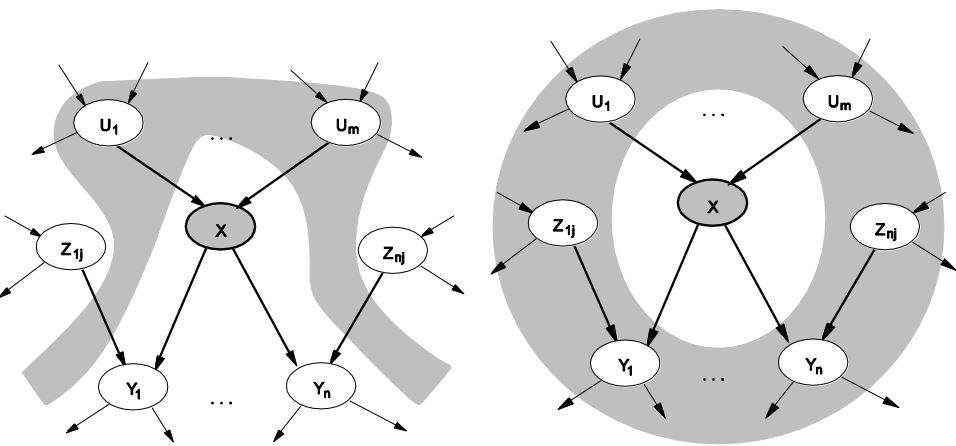
\includegraphics[width=\textwidth]{figures/markov-blanket.JPG}

	% TODO continue with chapter 14, slide 18
	
\end{document}
